\section{On Software Engineering}\label{sdp}
The software engineering lifecycle is host of several key process areas defined
for efficient organizations. We will discuss the properties and processes used
in software development and hour our proposed model fits in to this process.

\subsection{Properties of Software}\label{software_props}
There are key attributes about software and documentation that make them 
intrinsically different from other fields of engineering. These areas 
distinguish software engineering from traditional engineering in a way that 
complicates the process for safety-critical organizations. These unique
differences (1) make it difficult to identify software as a ``product'' liable
under the strict liability standard and (2) discourage sound documentation and
commenting practices.

\subsubsection*{Material Costs}

There are no upfront material costs to begin software implementation. No
specialized tools or equipment are necessary for the development of software.
Generic, over-the-shelf hardware like personal computers can be used to produce
tremendous feats in software engineering. In fact, Google, Inc. started by using
commodity machines to build what is now one of the most advanced search tools 
in computing \cite{Google}.

Because of this absence of material cost, it is easier for software engineers to
neglect to use certain precautions or care since there is no notion of immediate
damage of expensive equipment or loss due to injury. For example, an industrial
contractor may be dealing with expensive pieces of machinery when he installs
equipment for clients. This engineer would use extreme caution when working with
the machine, making repairs, or tooling with devices. He may even be working off
of very formal blueprints, instruction manuals, and installation documents. This
degree of formality is rarely seen in the software industry because no such
formal standard exists.

\subsubsection*{Product Replication}\label{software_product}
Since software is entirely digital, it is easily replicated. This means that
there is no chance that a copy of software can ever be a diversion from the
original design. A bug found in any particular instance of a software program
will exhibit itself in all copies of that piece of software, including the
``original''. This is because the formal design of the software \textit{is} the
product. This property of software makes it extremely difficult to classify
software defects as strict products liable.

\subsubsection*{Fast Turnaround}

More and more clients are demanding speed in implementation. Software developers
often deliver what is requested of them for immediate profit over long-term
gain, but what they deliver is a rushed, potentially unsafe product. This
mentality spreads throughout the organization. Stakeholders see no immediate
benefit from quality documentation. In addition, development teams will often
deliver implementations that satisfy specification, leading clients to expect
this level of performance all of the time. Because of this, developers are
indirectly discouraged to produce quality documentation because investors will
see this time spent as an unnecessary cost.

\subsubsection*{Testability}

Documentation is not testable. By their very nature, documentation and code
comments are open-ended artifacts with few restrictions or templates. This makes
it very difficult to validate the sufficiency of the documents created and
enforce an attitude of producing quality documents.

\subsubsection*{Bugs}

\begin{figure}
\singlespacing
\makebox[\textwidth]{\hrulefill}
\begin{lstlisting}
for (int i = 0; i < limit; i++)
{
  value = value * 1;
}
\end{lstlisting}
\makebox[\textwidth]{\hrulefill}
\doublespacing
\caption{Logic errors in C code}
\label{fig:logic_bug}
\end{figure}

Defects in software, commonly referred to as ``bugs'', manifest themselves in
different ways: (1) syntax errors, (2) runtime or execution errors, and (3)
logic errors.

Syntax errors occur when a software developer makes a mistake by 
typing incorrect symbols, tokens, or characters in the source code. These types
of errors or normally detected by the code-editing environment before errors
propagate.

Runtime errors are slightly less obvious than syntax errors because they do not 
exhibit flaws until the program is executed. A run-time error occurs when input
values or data types do not agree with the expected computation that is
currently executing (e.g. dividing by a zero or treating a string of characters
as if it were a number). Runtime errors are usually easy to identify because
they cause the execution environment of the program to halt. A thorough testing
phase will be able to catch most runtime errors.

The presence of logic errors in software code constitutes a chief difference
between software engineering and other, more physical engineering disciplines.
Logic errors occur when a developer's intention is not perfectly exhibited by
the code. A logic flaw can occur even if the code is entirely syntactically
correct. The program will compile and run as normal, and valid values for
variables will occur within expected ranges most of the time, but the program
will not behave as expected. Consider the hypothetical code snippet listed in
Figure \ref{fig:logic_bug}. In this example, the developer probably intended to
increment the variable \verb!value! by one each iteration of the loop. But
instead of using the addition \verb!+! symbol, he used the multiplication
\verb!*! symbol. This is syntactically correct code and the values of the
variables will appear within range, but the program will definitely not behave
as the developer intended it to.

Most errors in mechanically engineered machines are detectable. Engineers can
test physical flaws in their components and the system will exhibit them if they
are not repaired. Because there are no physical components in software,
software engineers must use extra precaution in other areas of the software
development lifecycle to compensate for this testability handicap.

\subsection{The Software Development Process}

In order to build a quality software systems, many organizations follow a
formal, methodological approach to the development process. Our solution relies
heavily on mature software processes and developers conforming to them. The
development process is described in general below, but more specifically in 
\cite{Royce1970}, \cite{Boehm1986}, \cite{CMM11}, and \cite{Kehoe1996}.

\subsubsection{Waterfall Model}\label{waterfall}
\begin{figure}[t]
\begin{center}
\includegraphics[scale=0.7]{images/waterfall.eps}
\end{center}
\caption{Waterfall Model of the Software Process}
\label{fig:waterfall}
\end{figure}
The original treatment of the waterfall model appears in \cite{Royce1970} and
describes a specification-driven approach to software development. Figure
\ref{fig:waterfall} shows different phases that flow steadily downwards (like a
waterfall). The model stresses a sequential occurrence of events in software
development, but also includes an iterative treatment to account for the 
evolving software development process.

Under the waterfall model, our solutions fits specifically in the ``coding''
cycle. Our strategy augments this phase with iterative commenting and
collaboration with legal analysts during development to ensure that current
implementation efforts exhibit social responsibility. For more information on
the waterfall model, see \cite{Royce1970}.

\subsubsection{Spiral Model}\label{spiral}
\begin{figure}[t]
\begin{center}
\includegraphics[scale=0.7]{images/spiral.eps}
\end{center}
\caption{Spiral Model of the Software Process}
\label{fig:spiral}
\end{figure}

The spiral model, as described in \cite{Boehm1986}, builds on refinements made
to the waterfall model. Boehm explains that the software process as an iteration
of four phases of activity -- shown as quadrants -- which can be retrofitted to
particularize to a variety of methods and approaches. As illustrated in Figure
\ref{fig:spiral}, the radial dimension represents the cumulative costs incurred
in accomplishing the steps to date while the angular dimension represents the
progress made in completing each spiral.

Notice that each rotation around the spiral begins with objectives,
consideration of alternatives, and the constraints on the system so (cost,
schedule, interface, etc.). According to Boehm's model, software developers
should take risks into consideration and these considerations should be
documented. Our model agrees with the spiral model and provides additional
information for risk analysis by generating more substantial data during the
development quadrant. For more information on the spiral model, refer to
\cite{Boehm1986}.
